% Chapter Template

\chapter{Proposed Methodology I} % Main chapter title

\label{chp:proposed1} % Change X to a consecutive number; for referencing this chapter elsewhere, use \ref{ChapterX}
This chapter presents a lightweight architecture for COVID-19 detection which is based on spatial kernel separability and residual connection. 

\begin{figure}[th]
    \centering
    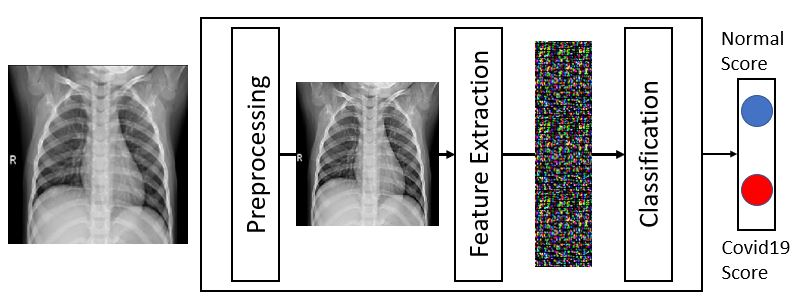
\includegraphics[height=40mm,width=8.0cm]{Figures/fig1.jpg}
    % \decoRule
    \caption{The phases of the proposed method I.}
    \label{fig1}
    \end{figure}

\section{Methodology I}
In this section, a  proposed  method I to detect COVID-19 disease from chest X-Ray images is presented. The proposed method exploits CNN model to classify the input chest X-Ray image to one of two categories; normal case or Covid-19 case. The proposed  method I consists of three phases: preprocessing, feature extraction, and classification. The proposed method phases are shown in Fig.\Ref{fig1}. 

\subsection{Preprocessing Phase}

The preprocessing phase is responsible for resizing and normalizing the  input  chest X-Ray images. The pre-processing phase is employed to maintain the numerical stability of the model and reduce the co-variance shift \cite{lecun1989handwritten}. In addition, this phase leads the learning model of CNN model to reduce  the required overhead to adapt to the different scales of different features of the input data. Reshaping size is determined empirically. The input  chest X-Ray image is re-sized and then adapted and normalized to a normal distribution as follows:

\begin{equation}
Y := \frac{x_i - \mu_{\mathcal B}}{\sqrt{\sigma_{\mathcal B}^2 + \epsilon}}
\label{eq1}
\end{equation}
where $\mu$ and $\sigma$ is the mean  and standard deviation of chest X-Ray image (X), respectively.

After re-sizing the input chest X-Ray image, the input image is normalized to have a zero mean and unit standard deviation. Then,  the image can be scaled and shifted with a normalization parameter which is determined and adapted by the training dataset during the training process according to the following equation: 

\begin{equation}
Z := w_1 Y + w_2
\label{eq2}
\end{equation}
where $w_1$ and $w_2$ are a trainable parameter.

Unlike the  normalization method presented in \cite{ioffe2015batch}, the batch normalization process presented in this paper has $z$-score normalization parameter that is used in both training and validation phases.


\subsection{Feature Extraction and Classification}

CNN models achieved an outstanding success in image recognition \cite{lecun2015deep}. This phase  is responsible for extracting spatial features from the normalized chest X-Ray image using a tailored CNN model.  This phase is based on learning the CNN model by the input preprocessed chest X-Ray images. The design of the tailored CNN model is described as follows: 

\subsubsection{Separable CNN kernels}
\begin{figure*}
\begin{center}
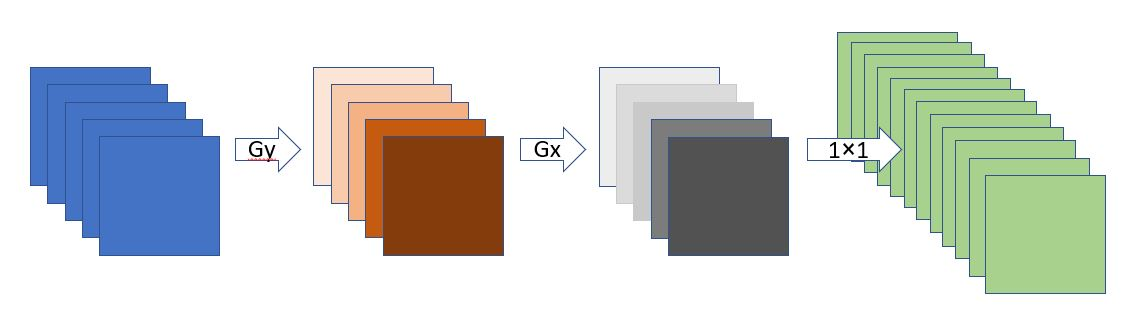
\includegraphics[height=33mm,width=14.0cm]{Figures/fig2.jpg}
\caption{Separable convolution  $Gy$ and $Gx$ have kernel size of $M\times1$ and $1 \times M$. The combination of these kernels is approximately a $M\times M$ kernel  and depth wise convolution are applied by a $1\times1$ convolution. The output depth  is padded with zeros to have the same spatial size of  $Gy, Gx$. $Gy, Gx$ are performed channel wise. }
\label{fig2}\end{center}\end{figure*}


    
Kernel separability\cite{rigamonti2013learning} \cite{szegedy2017inception} is based on decomposing a 2D convolution kernel to linear combinations of two 1D vectors which leads to a large reduction in  the total number of resulting parameters. For example, a 2D kernel of size $9 \times 9$ has a total number of $9^2 = 81$  trained parameters. Whereas in the case of separating this 2D kernel to  linear combinations of two 1D vectors of sizes $9 \times 1$ and $1 \times 9$, this results in a total number of  $9 + 9 = 18$ trained parameters. As a consequence, kernel separability reduces the number of CNN model operations (such as the multiplication and the addition). A  2D kernel of $k \times k$ applied for 2D signal with spatial dimensions of $ M \times N$ has a total number of  $(N-4)(M-4)\times k^2$ operations but in case of  applying kernel separability  yields $2(N-4)(M-4)k$ operations. The flow of separated convolution operations are summarized in Fig. \ref{fig2}. Fig. \ref{fig3} represents the structure, denoted by Separated Convolutional Layer, used in the proposed method with kernel size of $(M\times N)$ and satisfying the convolutional kernel separability. Separated Convolutional Layer is composed of three consecutive layers. The first convolutional layer has a kernel size of $(M\times1)$ and the number of convolutional neuron and  filters are equal to the number of channels as the input feature map and the convolution operations are performed in a channel wise. The second layer  operates in the same way as the first layer but it has a kernel of size $(1\times M)$. The third layer is the convolutional layer with kernel of size $(1\times1)$ and number of convolutional neuron is $N$. The collaboration of the three layers are  connected to preform similarly to the convolutional layer with kernel size of $(M\times M)$ and number of neuron and filter are the same as $N$ but with large difference in the performance.


\begin{figure}
    \begin{center}
    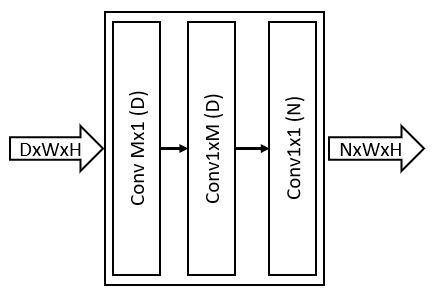
\includegraphics[height=34mm,width=7.0cm]{Figures/fig3.jpg}
    \caption{Separated Convolutional Layer}{ composed of three consecutive layers. The first Convolutional layer has a kernel size of $(M\times1)$ and $D$  convolutional neuron. The second layer  operates in the same way as the first layer but it has a kernel of size $(1\times M)$ and $D$ convolutional neuron. The third layer is the convolutional layer with kernel of size $(1\times1)$ and number of convolutional neuron is $N$.}
    \label{fig3}
    \end{center}
    \end{figure}

\subsubsection{ Batch Normalization and  Activation function}

In the proposed method linear separable convolutional kernels are followed by a batch normalization and an activation function. Rectified Linear Unit (ReLU) \cite{he2015delving} is a nonlinear activation that allows the network to fit and approximate highly non-linear datasets distribution. The proposed method employs the batch normalization which is described in \cite{ioffe2015batch}. 

Batch Normalization \cite{ioffe2015batch} reduces internal covariate shift produced as a result of  moving between layers during the feedforward procedure \cite{ioffe2015batch}. Batch Normalization makes the loss landscape smoother and reduces the number of saddle points \cite{santurkar2018does} which allows to use higher learning rates. Using a higher learning rate makes the network training  faster\cite{ioffe2015batch}. Batch normalization reduces the vanishing gradient problem and exploding gradient problem as it makes the resulted activation scale independent from the trainable parameter scale\cite{ioffe2015batch}. Batch normalization has the effect of regularization because of the inherited randomness when selecting the batch sample\cite{ioffe2015batch} which help the generalization to unseen chest X-Ray image.

\subsubsection{ Deep and larger receptive field Network design}

Deeper convolutional neural network design is a very important task for any image recognition task \cite{he2016deep}. Training a deeper network is very expensive and has many challenges such as vanishing gradient problem, exploding gradient problem, and degradation problem \cite{he2016deep}. Exploding gradient problem occurs  when the  gradient update becomes very large (approaching infinity) resulting in the network diversion. Vanishing gradient problem occurs when the  gradient update becomes very small (approaching zero) resulting in preventing the parameter update for early layers\cite{ioffe2015batch} and preventing the network to learn new patterns. Batch normalization \cite{ioffe2015batch} and the use of ReLU activation function \cite{krizhevsky2012imagenet} alleviate these two problems.

The deep layers of CNN networks sometimes need to  approximate the identity function which is not a simple task especially  with the existence of a non-linear functions. Residual connection\cite{he2016deep} overcomes this problem by using skip connection as shown in Fig. \ref{fig4}.
Fig. \ref{fig4} represents the building block layer of the feature extraction phase, denoted by stack of Residual Separated Block  (RSB). RSB consists of four layers of separated convolutional layers, each layer is followed by a batch normalization and an activation function. It has an output of depth $N$ where each sublayer produces an output of depth $N/4$ which is concatenated at the end of the layer to produce a depth  $N$. RSB produces a feature map that includes both low level features and high level features.

\begin{figure*}
\begin{center}
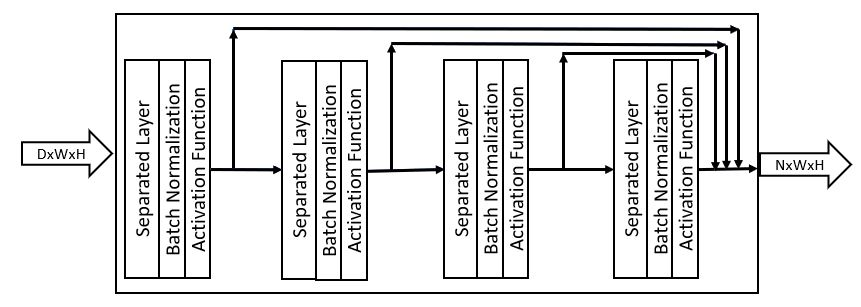
\includegraphics[height=38mm,width=14.0cm]{Figures/fig4.jpg}
\caption{The stack of residual separated block  (RSB) consists of four layer of separated convolutional layer each of which is followed by batch normalization and activation function.}
\label{fig4}
\end{center}
\end{figure*}

\begin{figure*}
    \begin{center}
    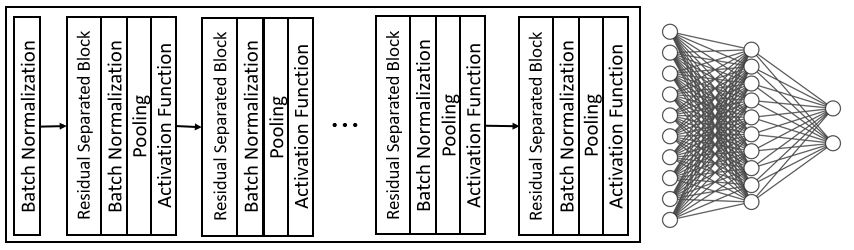
\includegraphics[height=37mm,width=14.0cm]{Figures/fig5.jpg}
    \caption{The complete proposed tailored CNN architecture.}
    \label{fig5}
    \end{center}
    \end{figure*}
    
Unlike the traditional neural network, which is fully connected to the previous layer, convolutional neural network is connected locally to a local region of the previous feature map. This introduces the concept of the network receptive field \cite{luo2016understanding}. Receptive field should be large enough to capture large patterns in the input chest X-Ray image. Therefore, any consecutive convolutional layers in the proposed method without a pooling layer in between a larger kernel size is used in one of them. Residual Separated block, RSB, in Fig. \ref{fig4} may have kernel sizes of 3, 5, 7, and 9, respectively.\\
Fig. \ref{fig5} Represent a complete CNN architecture.

\section{Summary}
In this chapter a lightweight CNN architecture is proposed for COVID19 detection. Proposed architecture is based on spatial separability of the convolutional kernel to enforce the learning of linear kernels. The proposed architecture consists of separated kernels convolutional layers that is connected by a residual connection. The proposed architecture uses batch normalization to maintain the network stability during the training process.
